\documentclass[12pt]{extarticle}
\usepackage[utf8]{inputenc}
%\usepackage{cite}
\usepackage[autolang=other,backend=biber,dateabbrev=false,sorting=none]{biblatex}
\usepackage{graphicx}
\usepackage{subcaption}
\usepackage{amsmath}
\usepackage{pdfpages}
\usepackage{listings}
\usepackage{float}
\usepackage[format=plain,
            labelfont={bf},
            textfont=it]{caption}
\lstset{
basicstyle=\fontsize{11}{13}\selectfont\ttfamily.
}

\addbibresource{ra.bib}

\title{CSM: Project Initiation}
\author{
Odysseas Karanikas\\
\texttt{odysseas.karanikas@rwth-aachen.de}
\and
Mann, Daniel\\
\texttt{daniel.mann@rwth-aachen.de}
\and
Daniel Rein\\
\texttt{drein99@outlook.de}
}

\date{April 2019}

\begin{document}

\maketitle

\section{Introduction}

\section{Functional Requirements}

The planned software can be understood as a mapping of a given input to an output. In our case, the input is an XES log file and one or more views and the output is a state chart. Since this function is our core feature it is important to discuss the details of input and output.

\subsection{Input}

The initial input of our software will be an XES file. XES stands for extensible event stream. It is a standard format for the representation of causally linked and ordered events and makes use of the XML format \cite{xes}. Generally, the structure of an XES file includes a trace and an event element where an event is a subelement of a trace. An event can contain attributes such as a timestamp, a name and other indivually specified properties. An excerpt of an XES file can look as follows\footnote{Usually an XES file contains additional metadata and definition of elements and attributes which we omitted in our example.}:

\begin{lstlisting}
<trace>
    <string key="concept:name" value="Trace number one"/>
    <event>
        <string key="concept:name" value="Register client"/>
        <string key="system" value="alpha" />
        <date key="time:timestamp" 
            value="2009-11-25T14:12:45:000+02:00" />
        <int key="attempt" value="23">
            <boolean key="tried hard" value="false" />
        </int>
    </event>
    <event>
        <string key="concept:name" value="Mail rejection"/>
        <string key="system" value="beta" />
        <date key="time:timestamp" 
            value="2009-11-28T11:18:45:000+02:00" />
    </event>
</trace>
\end{lstlisting}

A trace represents a closed and ordered process in the system while events depict stages or key points in the process. For example in an insurance company, one could consider all milestones of an insurance case as events belonging to the same trace. Another case would then necessitate another trace.

In our case the event log will have a particular semantic. We will understand the events as states that a process goes through where these states are spread in time. That is every event has a duration attribute denoting how long a given process, represented by a trace, spend in the corresponding event. To make this clearer, we will take the example of a grocery store. A trace and thus a process corresponds to a customer pathing through the store. On his way through the store he will go through different locations which will be his states. These locations can be the entrance ($S$), two different sections of the bakery ($B_1$ and $B_2$), two different subsections of the beverage section ($G_1$, $G_2$) and finally the cash register ($P$) and the exit section $E$. A possible log file can look as follows:

\begin{lstlisting}
Trace	State   Duration
1 	S   	1
1 	B_1 	3
1 	G_2 	4
1 	P   	5
1 	E   	1

2 	S   	1
2 	G_1 	3
2 	P   	4
2 	E   	1

3 	S   	1
3 	E   	1

4 	S   	1
4 	B_2 	3
4 	P   	3
4 	E   	1
\end{lstlisting}

Here we chose a different more simple representation that captures the order of states, their respective duration and their affiliated trace.

The log file is not the only input we expect. The user should furthermore be able to create views as discussed in the Use case section. A view is an explicitly non-injective mapping from the initial state space to the target state space. Both the mapping the target state space are determined by the user and comprise the view. We use the example of the grocery store from above and give two example views:

\begin{lstlisting}
States 	View1	View2

S	S	S'
B_1	B	S'
B_2	B	S'
G_1	G	G
G_2	G	G
P	E'	E'
E	E'	E'
\end{lstlisting}

\subsection{Output}

In the Feasibility Study of the our Project Initiation we already discussed some structure of the output. In general, our output will be a set of graphs depicted in different views. One of these views will be the original view that is computed from the log file directly. Nodes in this graph represent states in the logs. Each node contains the name of the state, the average duration and the total number of occurrences in the event log. The average is computed over all occurrences.
The edges represent state transitions. When in a trace, one state directly follows another one then their corresponding nodes are to be connected by a directed edge where this edge points to the later, successor state. Each such transition is annotated with the relative frequency of transitions to the target state given the total number of occurrences from that state \textbf{or the total number of outgoing transitions from that state}. This is illustrated in Figure \ref{fig:ogview}.

\begin{figure}[htbp]
    \centering
    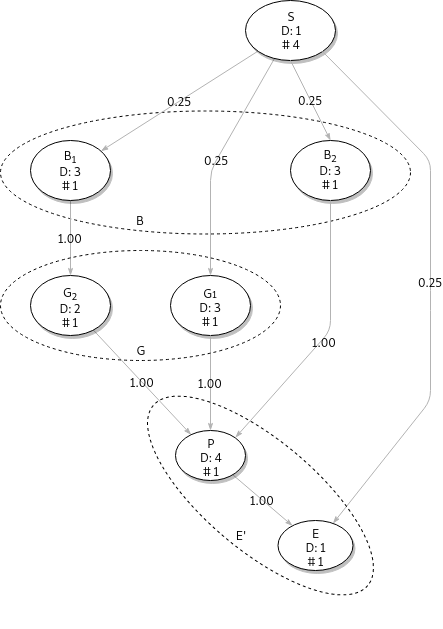
\includegraphics[width=0.7\textwidth]{Diagrams/Statecharts/statemachine.png}
    \caption{An example output following the log presented above. We see that the transition from $S$ to $B_1$ is annotated by the numeric value $0.25$. This follows from that fact that $B_1$ followed $S$ in a fourth of the times. The dashed ellipses represent a possible view on could choose.}
    \label{fig:ogview}
\end{figure}

The other output graphs correspond to the views as specified in the subsection on the input. In a view, a number of states can be lumped into the same state. In the above example view 1, the states $B_1$ and $B_2$ are combined to the state $B$. The resulting state holds again an average duration time. We imagine two different possibilities for the computation of this value. Either we could average over all occurrences of every state in the combined state or for every trace sum up the total duration time in the combined state and then average over all traces\footnote{We deem the latter option to be more meaningful but leave the discussion to be open until our advisor has been consulted about this issue.}. The total number of occurrences of the composite state is the sum of the number of occurrences of every component state. 



We shall investigate the transition frequencies of the composite states further. Let $\Omega$ denote the state space. We consider a transition from the composite states $S \subset \Omega$ to $T \subset \Omega$ where we understand both states as sets of basic states. The number of transitions from states all substates of $S$ to all substates of $Q$ is then the number
\[ 
    \sum_{(s,q) \in S \times Q} N(s,q)
\]
where $N(s,q)$ denotes the number of transitions observed between the original, raw states $s$ and $q$. The relative frequency of transitions between the composite states $S$ and $Q$ is then given by the above sum divided by the number
\[
    \sum_{(s,t) \in S \times \Omega} N(s,t)
\]
of outgoing transitions from the lumped state $S$.

To illustrate this procedure let us consider the partitioning chosen in figure \ref{fig:ogview}. Here a we have the state space $\Omega = \{ S, B_1, B_2, G_1, G_2, P, E \}$\footnote{Mind that $S$ is here a basic state while in our notation about $S$ is composite}. The composite states we chose in the first example view are $B := \{ B_1, B_2 \} $, $G = \{ G_1, G_2 \}$ and $E' = \{ P, E \}$. The graph is then transformed according to the rules discussed above, yielding the graph in figure \ref{fig:view1}.

\begin{figure}[hb]
    \centering
    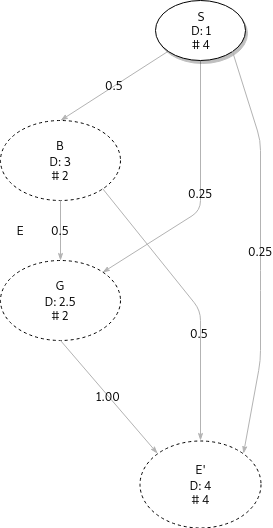
\includegraphics[width=0.5\textwidth]{Diagrams/Statecharts/statemachine_view1.png}
    \caption{State composition of figure \ref{fig:ogview} has been applied and the transitions and state informations adjusted according to the rules discussed in the text.}
    \label{fig:view1}
\end{figure}

Another example for how a view is supposed to transform the graph we can find in figure \ref{fig:pandv}.

\begin{figure}[H]
    \centering
    \begin{subfigure}[b]{0.6\textwidth}
        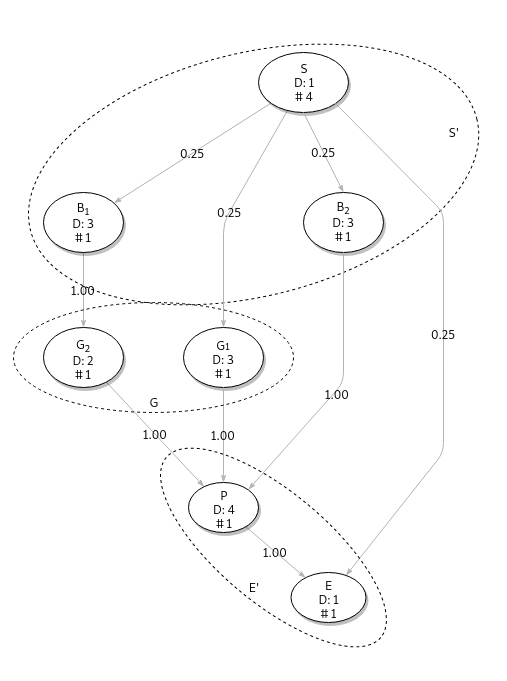
\includegraphics[width=\textwidth]{Diagrams/Statecharts/statemachine_preview2.png}
        \caption{State chart with a differen partitioning of states.}
        \label{fig:preview2}
    \end{subfigure}
    \\ %add desired spacing between images, e. g. ~, \quad, \qquad, \hfill etc. 
      %(or a blank line to force the subfigure onto a new line)
    \begin{subfigure}[b]{0.45\textwidth}
        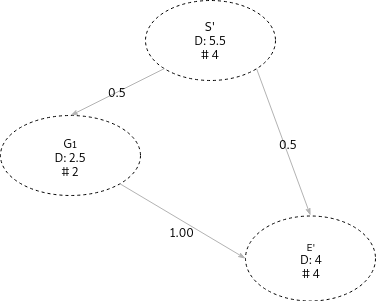
\includegraphics[width=\textwidth]{Diagrams/Statecharts/statemachine_view2.png}
        \caption{The resulting view.}
        \label{fig:view2}
    \end{subfigure}
    \caption{A different selection of composite states in the same example and the requirement for the output graph.}
    \label{fig:pandv}
\end{figure}

\end{document}